% !TEX root = ./Vorlesungsmitschrift DIFF 2.tex  
\lecture{Do 09.07. 10:15}{}
\chapter{Integration auf Untermannigfaltigkeiten}
\begin{erinnerung*}[\ordinalnum{14} Vorlesung]
  \begin{figure}[H]
    \centering
    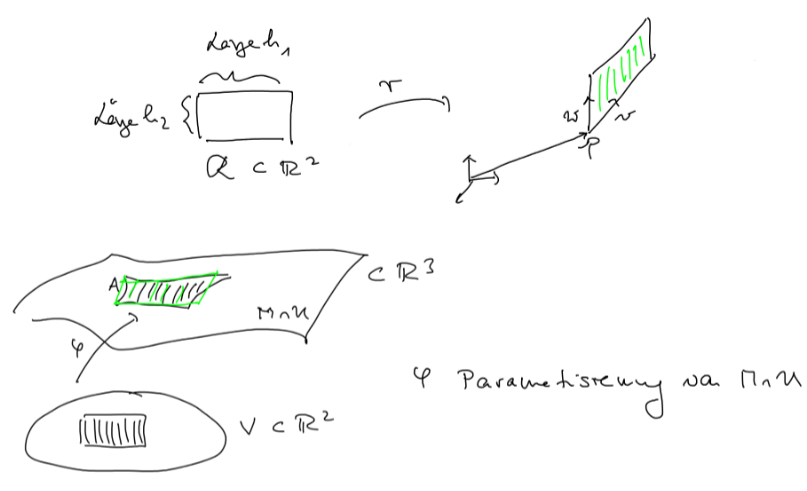
\includegraphics[width=\linewidth]{flaeche_unter_mannigfaltigkeit}
    \label{fig:flaeche_unter_mannigfaltigkeit}
  \end{figure}
  Flächeninhalt von \( \varphi(\mathcal{R})\approx \sqrt{\det-{g_{\varphi}(t_0)}}\text{Fläche}(\mathcal{R}) \). (\( \det-{g_{\varphi}(t_0)} \) heißt Gramsche Determinante) mit dem metrischen Tensor \( g_{\varphi} \)
  \begin{align*}
    \scalarproduct{v}{v}_a=\sum_{i}\sum_{j}v_i w_j\braceannotate{\definedas \p*{g_\varphi}_{ij}(t_0)}{\scalarproduct{\partial_i \varphi(t_0)}{\partial_j \varphi(t_0)}_\text{E}}\\
    \scalarproduct{v}{w}_a=\scalarproduct{v}{w}_{\text{E}}\quad \text{für}\logicspace a\in M\cap U,\logicspace v,w\in \tangentialraum{M}.
  \end{align*}
  \thref{berechnung_gramsche_determinante}: \( \determinant{g}(t_0)=\sum_{\mathclap{i_1<\dotsb<i_d}}\p*{\determinant{\totalderivative{\begin{pNiceMatrix} \varphi_{i_1} \\ \Vdots \\ \varphi_{i_d} \end{pNiceMatrix}}}(t_0)}^2 \).

  \thref{parameterwechsel_metrischer_tensor}: Unter Parameterwechsel (\vgl \ref{parameterwechsel}) verhält sich der metrische Tensor wie folgt
  \begin{equation*}
    \explain[big]{\text{\bzgl \( \psi\maps \tilde{V}\to M\cap \tilde{U} \) berechnet}}{g_{\psi}}=\transpose+{\totalderivative{\Phi}(s)}\explain{\text{\bzgl \( \varphi\maps V\to M\cap U \) berechnet}}{g_{\varphi}}\totalderivative{\Phi}(s)
  \end{equation*}
  mit \( \Phi=\inverse{\varphi}\circ \psi\maps \inverse{\psi}(M\cap U\cap \tilde{U})\to \inverse{\varphi}(M\cap U\cap \tilde{U})\).
\end{erinnerung*}
\begin{definition}\label{mannigfaltigkeit_integral}\index{Integration auf Untermannigfaltigkeiten}
  Sei \( M\subset \reals^n \) eine \( d \)-dimensionale Untermannigfaltigkeit. Es sei 
  \begin{enumerate}[label=\rechtsklammer{\alph*}]
    \item\label{mannigfaltigkeit_integral:globale_parametisierung} \( \varphi\maps V\to \reals^n \) eine globale Parametrisierung von \( M=\varphi(V) \) und \( f\maps M\to \reals \) eine Funktion, \emph{oder}
    \item\label{mannigfaltigkeit_integral:lokale_parametisierung} \( \varphi\maps V\to \reals^n \) eine lokale Parametrisierung von \( M\cap U \) und \( f\maps M\to \reals \) eine Funktion mit 
    \begin{equation*}
      \supp f=\abschluss{\set{x\in M|f(x)\neq 0}}\subset \varphi(V).
    \end{equation*}
    Dann heißt \( f \) über \( M \) integrierbar, falls
    \begin{equation*}
      t\mapsto f\circ \varphi(t)\sqrt{\determinant{g_{\varphi}(t)}}
    \end{equation*}
    über \( V \) integrierbar ist, und man setzt
    \begin{equation*}
      \Integrate{f(x)}{S(x),M}\definedas \Integrate{f\circ \varphi(t)\sqrt{\determinant{g_{\varphi}(t)}}}{t,V}.
    \end{equation*}
  \end{enumerate}
\end{definition}
\begin{bemerkung*}
  Mit der Transformationsformel und \thref{parameterwechsel_metrischer_tensor} sieht man schnell, das die Definition unabhängig von der gewählten Parametrisierung ist.
\end{bemerkung*}
\begin{folgerung}\label{berechnung_mannigfaltigkeit_integral_ueber_zerlegung_der_eins}
  Das Integral ist auf einer Untermannigfaltigkeit definiert (ohne die Einschränkungen \ref{mannigfaltigkeit_integral:globale_parametisierung} und \ref{mannigfaltigkeit_integral:lokale_parametisierung} in \thref{mannigfaltigkeit_integral}).
  \begin{figure}[H]
    \centering
    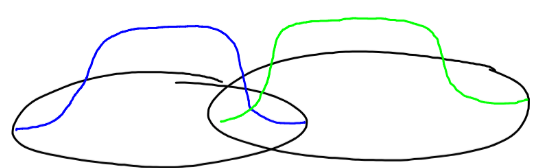
\includegraphics[width=0.5\linewidth]{mannigfaltigkeit_integral_unabhaengig_von_parametisierung}
    \label{fig:mannigfaltigkeit_integral_unabhaengig_von_parametisierung}
  \end{figure}
  \begin{equation*}
    \Integrate{f\circ \varphi(t)\sqrt{\determinant{g_{\varphi}(t)}}}{t,\inverse{\varphi}(A)}=\Integrate{f\circ \psi(t)\sqrt{\determinant{g_{\psi}(t)}}}{t,\inverse{\psi}(A)}.
  \end{equation*}
  Wir schreiben daher \( \Integrate{f}{S,M} \), auch wenn \ref{mannigfaltigkeit_integral:globale_parametisierung} und \ref{mannigfaltigkeit_integral:lokale_parametisierung} nicht erfüllt sind. 

  Berechnung des Integrals:\\
  Sei \( \set{\rho_j}_j \) eine Zerlegung der Eins, also
  \begin{equation*}
    \sum_{j=1}^{\infty}\rho_j(a)=1 \quad \forall a\in M,\quad \rho_j\in \stetigefunktionen[\infty], \logicspace\rho_j\geq 0
  \end{equation*}
  \sd für jedes \( j \) gilt \( \supp \rho_j\subset  \) ein Kartengebiet in \( M \).
  Existenz: Existenz von Abschneidefunktionen \( \psi \) in \( \reals \) \timplies Existenz von Abschneidefunktionen in \( \reals^n \)
  \begin{equation}
    \Psi(x)\definedas \psi\p*{\euclidiannorm{x}},\quad x\in \reals^n
  \end{equation}
  \timplies Wenn \( M \) durch 
  \( \p*{\varphi_i\maps U_i\to V_i}_{i\in I} \)
   beschrieben wird,
    also \tforall \( a\in M \) \texists \( i\in I \) \sd \( a\in \varphi_i(U_i) \), betrachte Partition der Eins \( \Set{\tilde{\rho}_j}_{j\in J} \) mit: Zu \( j \) \texists \( i\in I \) \sd \( \supp \tilde{\rho}_j\subset U_i \) und setze \( \rho_j=\tilde{\rho}_j\circ \inverse{\varphi_i} \).
  \begin{figure}[H]
    \centering
    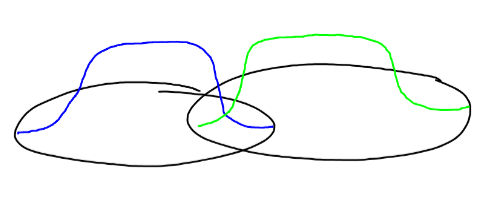
\includegraphics[width=0.5\linewidth]{berechnung_mannigfaltigkeit_integral_ueber_zerlegung_der_eins}
    \label{fig:berechnung_mannigfaltigkeit_integral_ueber_zerlegung_der_eins}
  \end{figure}
  Dann ist 
  \begin{equation*}
    \Integrate{f}{S,M}=\sum_{j\in J} \Integrate{\rho_j f(x)}{S,M}.
  \end{equation*}
  \timestamp{12:06--16:30 \tto weitere Erklärungen im Audio}
\end{folgerung}
\begin{ergaenzung*}
  \begin{enumerate}[label=\rechtsklammer{\arabic*}]
    \item Sei zunächst \( M\subset \reals^n \) offen. \( \rho_j f \) auf \( M \) integrierbar \tiff \( \rho_j \abs{f} \) auf \( M \) integrierbar.
    Sei also \( \rho_j\abs{f} \) auf \( M \) integrierbar. Es ist
    \begin{equation*}
      \sum_{j=1}^{K}\rho_j \abs{f}\goesupto \abs{f}.
    \end{equation*}
    Ist \( \sum_{j=1}^{\infty}\Integrate{\rho_j \abs{f}}{S}<\infty \), können wir mit Beppo-Levi schließen, dass \( \abs{f} \) integrierbar ist.

    Wegen \( \abs*{\sum_{j=1}^{K}\rho_j f}\leq \abs{f} \) (\( \triangle \)-Ungleichung) folgt mit Lebesgue, dass \( f=\sum_{j=1}^{\infty}\rho_j f \) integrierbar ist und gilt
    \begin{equation*}
      \Integrate{f}{x,M}=\sum_{j=1}^{\infty}\Integrate{\rho_j f}{x,M}.
    \end{equation*}
    Das zeigt auch gleich die Unabhängigkeit von der Wahl der Teilung der Eins.
    \item Ist \( \varphi\maps U\to M \) globale Parametrisierung von \( M\) betrachte \( F\definedas f\circ \varphi \sqrt{\determinant{g_{\varphi}}} \). Es ist \( F \) auf \( U \) integrierbar \tiff \( f \) auf \( M \) integrierbar.
    \item Mithilfe von \( \tilde{\rho}_j=\rho_j \circ \phi_{i(j)} \) ziehen wir das oben bewiesene auf die verschiedenen Koordinatenbereiche zurück: \( \rho_j f \) auf \( M \) integrierbar \tiff \( \tilde{\rho}_j F \) auf \( U_{i(j)} \) integrierbar.
  \end{enumerate}
\end{ergaenzung*}
\begin{beispiel*}[das ohne Zerlegung der Eins auskommt]
  \( M=\text{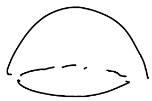
\includegraphics[height=\baselineskip]{immersion_halbkugel}} \), \( M=\varphi(D) \), \( D=\set{x^2+y^2<1} \), \( \varphi(x,y)=\transpose{(x,y,\sqrt{1-x^2,y^2})} \).

  \( f(a)=1\quad \forall a\in M \) \timplies Wir berechnen die Oberfläche.
  \begin{gather*}
    g_{\varphi}(a)=\begin{pNiceMatrix} 1-x^2 & xy \\ xy & 1-y^2 \end{pNiceMatrix}\frac{1}{1-x^2-y^2},\logicspace \determinant{g_{\varphi}}=1,\\
    \partial_1 \varphi=\p*{1,0,\frac{-x}{\sqrt{1-x^2-y^2}}},\quad \partial_2\varphi=\p*{0,1,\frac{-y}{\sqrt{1-x^2-y^2}}},\\
    \Integrate{}{S,M}=\Integrate{}{{(x,y)},D}\explain{\text{Schule}}{=}2\pi\explain{\text{\s unten}}{=}\Integrate{}{{(x,y)},\text{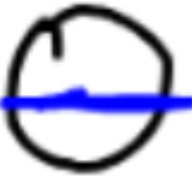
\includegraphics[height=0.3\baselineskip]{kreis_ohne_durchmesser}}}=2\Integrate{\Integrate{}{x,-\sqrt{1-y^2},\sqrt{1-y^2}}}{y,0,1}.
  \end{gather*}
  \begin{figure}[H]
    \centering
    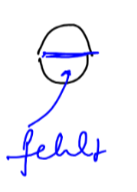
\includegraphics[width=0.1\linewidth]{kreis_ohne_durchmesser_anmerkung}
    \label{fig:kreis_ohne_durchmesser_anmerkung}
  \end{figure}
  Alternativ: \( \varphi\maps \ointerval{0}{2\pi}\times \ointerval{0}{\frac{\pi}{2}}\to \reals^3 \),
  \begin{figure}[H]
    \centering
    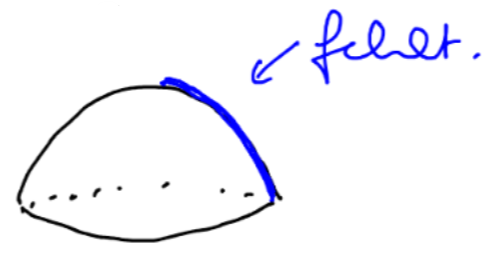
\includegraphics[width=0.3\linewidth]{halbkugel_ohne_radius}
    \label{fig:halbkugel_ohne_radius}
  \end{figure} 
  \begin{gather*}
    \varphi(a,\theta)=\begin{pNiceMatrix} \Cos{\alpha}\Sin{\alpha} \\ \Sin{\alpha}\Sin{\theta} \\ \Cos{\theta} \end{pNiceMatrix}, \quad g_\varphi(\alpha,\theta)=\begin{pNiceMatrix} \sin^2 \theta & 0 \\ 0 & 1 \end{pNiceMatrix}\\
    \Integrate{}{S,M}\explain{\text{\s unten}}{=}\Integrate{}{S,M\setminus \text{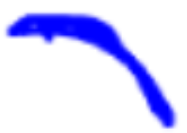
\includegraphics[height=0.3\baselineskip]{durchmesser}}}=\Integrate{\Integrate{\Sin{\theta}}{\theta,0,\frac{\pi}{2}}}{\alpha,0,2\pi}=2\pi.
  \end{gather*}
\end{beispiel*}
\begin{definition}\label{d_nullmenge}\index{\( d \)-Nullmenge}
  Sei \( d\in \reals_{>0} \). Eine Teilmenge \( N\subset \reals^n \) heißt \emph{Nullmenge zur Dimension \( d \)} (\( d \)-Nullmenge), falls \tforall \( \varepsilon>0 \) \texists  Würfel \( W_1,W_2,\dotsc \) mit Kantenlängen \( r_1,r_2,\dotsc \),  \sd \( N\subset \bigcup W_j \) und \( \sum r_j^d<\varepsilon \).
\end{definition}
\begin{bemerkungen}
  \begin{enumerate}\label{d_nullmenge_eigenschaften}
    \item Ist \( d=n \), liegt eine Nullmenge im Sinne von \thref{nullmenge} vor.
    \item Eine Teilmenge von \( \reals^d\times \zeroset \subset \reals^n \) ist genau dann \( d \)-Nullmenge in \( \reals^n \), wenn sie Nullmenge in \( \reals^d \) ist (im Sinne von \thref{nullmenge}), wobei hier \( N=\tilde{N}\times \set{0}\simeq \tilde{N} \), \( \reals^d\times \zeroset \simeq \reals^d \).
    \begin{proof}
      \begin{proofdescription}
        \item[\hin] Setze \( W_j^0\definedas W_j\cap \reals^d\times \zeroset \)\\
        \item[\rueck]  Fasse einen Würfel \( W_j\subset \reals^d\times \zeroset \) auf als den Schnitt eines Würfels \( \tilde{W}_j\subset \reals^n \) mit \( \reals^d\times\zeroset \).
      \end{proofdescription}
    \end{proof}
    \timestamp{25:45}
    \item \( M\subset N \), \( N \) \( d \)-Nullmenge \timplies \( M \) ist \( d \)-Nullmenge.
    \item Abzählbare Vereinigungen von \( d \)-nullmengen sind \( d \)-Nullmengen.
    \item Eine \( d \)-Nullmenge ist auch \( d' \)-Nullmenge für \( d'\geq d \).
    \item \label{d_nullmenge_eigenschaften:lipschitz_stetige_funktion_erhaelt_d_nullmenge}Ist \( \Phi \) lokal Lipschitz-stetig. \( \Phi\maps N\to \reals^m \), \( N\subset \reals^n \) \( d \)-Nullmenge, so ist \( \Phi(N) \) \( d\)-Nullmenge.
    \begin{proof}
      Der Beweis von \thref{lipschitz_stetige_funktion_bild_von_nullmenge_ist_nullmenge} überträgt sich direkt.      
    \end{proof}
    \item \begin{folgerung*}
      Jede \( d \)-dimensionale Untermannigfaltigkeit ist \( (d+1) \)-Nullmenge. \emph{denn}: \texists \( \Phi\maps U\cap M\to V\times \zeroset^{n-d} \) Diffeomorphismus.
    \end{folgerung*}
  \end{enumerate}
\end{bemerkungen}
\begin{satz}
  Seien \( f,g\maps M\to \reals \), \( M \) \( d \)-dimensionale Untermannigfaltigkeit \tsubset \( \reals^n \). Gelte \( f(x)=g(x) \) außer auf einer \( d \)-Nullmenge \( N \) und sei \( f \) über \( M \) integrierbar. Dann ist auch \( g \) über \( M \) integrierbar und es gilt
  \begin{equation*}
    \Integrate{f}{S,M}=\Integrate{g}{S,N}.
  \end{equation*}
\end{satz}
\begin{proof}
  Betrachte zunächst nur \emph{eine} Parametrisierung \( \varphi\maps \to M\cap U \). Dann stimmen die Funktionen \( f\circ \varphi \sqrt{\determinant{g_{\varphi}}}  \) und \( g\circ \varphi\sqrt{\determinant{g_{\varphi}}} \) außerhalb von \( \inverse{\varphi}(N)\subset V\subset \reals^d \) miteinander überein. \ref{d_nullmenge_eigenschaften:lipschitz_stetige_funktion_erhaelt_d_nullmenge} \timplies \( \inverse{\varphi}(N) \) ist \( d \)-Nullmenge (denn \( \inverse{\varphi} \)  ist wieder \( \stetigefunktionen[1] \), also lokal Lipschitz-stetig).
  
  Mit Hilfe einer Partition der Eins wie in \ref{berechnung_mannigfaltigkeit_integral_ueber_zerlegung_der_eins} folgt die Behauptung, da auch \( \rho_j\cdot f \) außerhalb von \( N \) mit \( \rho_j\cdot g \)
  übereinstimmt.
\end{proof}
\begin{folgerung*}
  Ist \( N \) \( d \)-Nullmenge \tsubset \( \reals^n \) und \( M \) \( d \)-dimensionale Untermannigfaltigkeit \tsubset \( \reals^n \) so ist
  \begin{equation*}
    \Integrate{f}{S,M}=\Integrate{f}{S,M\setminus N}.
  \end{equation*}
  Dies erklärt unsere Ergebnisse aus dem Beispiel unter \thref{berechnung_mannigfaltigkeit_integral_ueber_zerlegung_der_eins}.
\end{folgerung*}
\timestamp{33:00}
\begin{beispiel*}[Rotationsflächen]
  Sei \( r\maps I\to \rinterval{0}{\infty} \) stetig, \( I \) Intervall. Sei \( r \) zudem außerhalb einer endlichen Menge von Punkte in \( I \) \( \stetigefunktionen[1] \), \zb 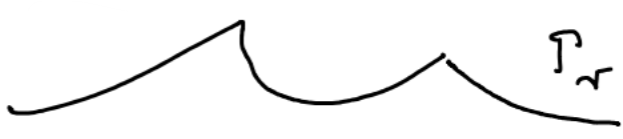
\includegraphics[height=\baselineskip]{fast_ueberall_c1}.

  Wir berechnen die Oberfläche (ohne \enquote{Deckel} + \enquote{Boden}) von
  \begin{equation*}
    M\definedas \Set{(x,y,z)\in \reals^3|x^2+y^2=r^2(z)}.
  \end{equation*}
  \begin{figure}[H]
    \centering
    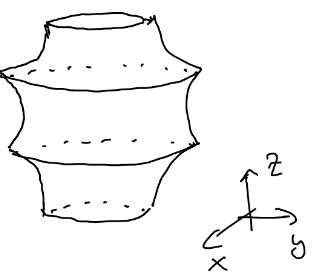
\includegraphics[width=0.5\linewidth]{rotationsflaeche_oberflaeche}
    \label{fig:rotationsflaeche_oberflaeche}
  \end{figure}
  \Obda betrachte nur glatte Abschnitte (denn die Kreise 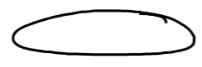
\includegraphics[height=\baselineskip]{rotationsflaeche_kreise}) sind \( 2 \)-Nullmengen.
  \begin{equation*}
    A=\Integrate{1}{S}=2\pi \Integrate{r(z)\sqrt{r'(z)^2+1}}{z,h_0,h_1},
  \end{equation*}
  denn:
  \begin{gather*}
    \varphi\maps \ointerval{0}{2\pi}\times \ointerval{0}{h}\to \reals^3\\
    \varphi(\alpha,z)=(r(z)\Cos{\alpha},r(z)\Sin{\alpha},z)\\
    g_{\varphi}(a,z)=\begin{pNiceMatrix} r(z)^2 & 0 \\ 0 & r'(z)^2+1 \end{pNiceMatrix}\\
    \sqrt{\determinant{g_{\varphi}}}=r(z)\sqrt{r'(z)^2+1}
  \end{gather*}
  \begin{beispiel*}
    \begin{figure}[H]
      \centering
      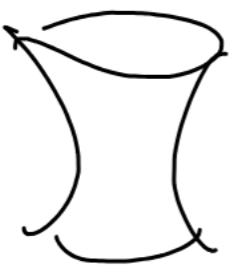
\includegraphics[width=0.2\linewidth]{wurzelrotationsflaeche}
      \label{fig:wurzelrotationsflaeche}
    \end{figure}
    \( r(z)=\sqrt{z^2+1} \), \( r'(z)=\frac{z}{\sqrt{z^2+1}} \)
    \begin{equation*}
      A=2\pi \Integrate{\sqrt{2z^2+1}}{z,-h,h}=2\pi\p*{\sqrt{2h^2+1}h+\frac{1}{\sqrt{2}\ArcSin+{\sqrt{2}h}}}.
    \end{equation*}
  \end{beispiel*}
\end{beispiel*}
\timestamp{37:10}
\section{Der Integralsatz von Gauß}
Integralsätze der Vektoranalysis sind von der Form
\begin{equation*}
  \int_V\dotsc=\int_{\randpunkte{V}}\dotsc,
\end{equation*}
wobei \( V \) \zb eine Untermannigfaltigkeit und \( \randpunkte{V}  \) ihr Rand (mal der topologische mal der geometrische).
\begin{erinnerung*}
  Sei \( G\subset \reals^n \) wegzusammenhängende, beschränkte \( n \)-dimensionale Untermannigfaltigkeit mit Rand. In diesem Fall stimmen der topologische Rand und der geometrische Rand miteinander überein. Sei \( h\maps U\to \reals^n \) eine lokale Beschreibung von \( G \) bei \( a\in \randpunkte{G} \), also 
  \begin{equation*}
    G\cap U=\set{x\in U|h(x)\leq 0},
  \end{equation*}
  wobei
  \begin{equation*}
    \randpunkte{G}\cap U=\Set{x|h(x)=0},
  \end{equation*}
  (also \( \randpunkte{G} \) ist \( (n-1) \)-dimensionale Untermannigfaltigkeit)
  (Alternative zu \thref{untermannigfaltigkeit_mit_rand}).

  Betrachte den \emph{äußeren Einheitsnormalenvektor}
  \begin{equation*}
    n_a\definedas \frac{\grad{h(a)}}{\norm{\grad{h(a)}}}
  \end{equation*}
  im Punkt \( a \).
  \begin{beispiel*}
    \( G=\Set{x\in \reals^n|\euclidiannorm{x}\leq 1} \) Vollkugel. \( \randpunkte{G}=\sphere{n-1} \), \( h(x)=\euclidiannorm{x}^2-1 \), \( n_a=\frac{a}{\norm{a}} \).
  \end{beispiel*}
  Verwende eine lokale Beschreibung von \( \randpunkte{G} \) als Graph einer \( \stetigefunktionen[1] \)-Funktion \( \varphi \)
  \begin{equation*}
    \randpunkte{G}\cap V=\Set{(x_1,\dotsc,x_{n-1},\varphi(x_1,\dotsc,x_{n-1}))|(x_1,\dotsc,x_{n-1})\in \tilde{U}}.
  \end{equation*}
  Dann ist (nach eventueller Umnummerierung)
  \begin{equation*}
    h(x',x_n)=x_n-\varphi(x')\quad x'\in \tilde{U}\subset \reals^{n-1 }
  \end{equation*}
  und
  \begin{equation*}
    n_a=\begin{pNiceMatrix} -\grad{\varphi(a')} \\ 1 \end{pNiceMatrix}\frac{1}{\sqrt{1+\norm{\grad{\varphi(a')}}^2}}\quad a=(a',a_n)
  \end{equation*}
  und \( \sqrt{\determinant{g_{\Phi}(x')}}=\sqrt{1+\norm{\grad{\varphi(x')}}^2} \)
  \begin{align*}
    \Phi(x')&=(x',\varphi(x'))\quad x'\in \tilde{U}\\
    \partial_j \Phi&=e_j+\partial_j \varphi e_n\quad 1\leq j\leq n-1.
  \end{align*}
\end{erinnerung*}
\begin{satz}[Integralsatz von Gauß]\index{Integralsatz von Gauß}\label{integralsatz_gauss}
  Sei \( G\subset \reals^n \) wegzusammenhängende, beschränkte \( n \)-dimensionale Untermannigfaltigkeit mit Rand. Sei \( n\maps \randpunkte{G}\to \reals^n \) das äußere Einheitsnormalenvektorfeld (das stetig ist). Sei \( U\supset G \) offen. Dann gilt für jedes \( \stetigefunktionen[1] \)-Vektorfeld \( X\maps U\to \reals^n \)
  \begin{equation*}
    \Integrate{\braceannotate{=\sum_{j=1}^{n}\partial_j X_j(x)}{\divergence{X(x)}}}{x,G}=\Integrate{\scalarproduct{X(x)}{n(x)}}{S(x),\randpunkte{G}}.
  \end{equation*}
\end{satz}
\timestamp{47:35}
\begin{figure}[H]
  \centering
  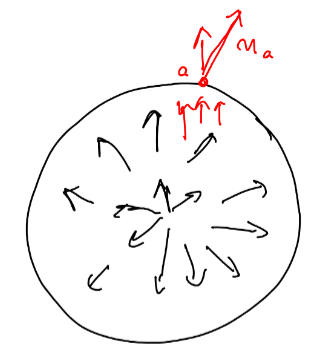
\includegraphics[width=0.5\linewidth]{divergenz}
  \label{fig:divergenz}
\end{figure}
\( \divergence{X} \) misst die \emph{Quellstärke}, denn: \( \totalderivative{X} \) misst wie sich \( X \) verändert. Eigenwerte von \( \totalderivative{X}(x_0) \): 
\begin{description}
  \item[Eigenwerte positiv] \tto in Richtung des zugehörigen Eigenvektors anwachsend (Quelle)
  \item[Eigenwerte negativ] \tto in Richtung des zugehörigen Eigenvektors schrumpfend (Senke)
\end{description}
Summe aller Eigenwerte \teq Maß für Quellstärke
\begin{equation*}
  =\Spur{\totalderivative{X}(x_0)}=\sum_{i=1}^{n}\partial_i X_i(x_0).
\end{equation*}